\documentclass[a4paper,12pt]{article}
\usepackage{amsmath}
\usepackage{pdfpages}
\usepackage[utf8]{inputenc}
\usepackage{hyperref}
\usepackage{listings}
\usepackage{xcolor}
\usepackage{fancyhdr}
\definecolor{codegreen}{rgb}{0,0.6,0}
\definecolor{codegray}{rgb}{0.5,0.5,0.5}
\definecolor{backcolour}{rgb}{0.95,0.95,0.92}

\lstdefinestyle{mystyle}{
    backgroundcolor=\color{backcolour},   
    commentstyle=\color{codegreen},
    keywordstyle=\color{blue},
    numberstyle=\tiny\color{codegray},
    basicstyle=\ttfamily\footnotesize,
    breakatwhitespace=false,         
    breaklines=true,                 
    captionpos=b,                    
    keepspaces=true,                 
    numbers=left,                    
    numbersep=5pt,                  
    showspaces=false,                
    showstringspaces=false,
    showtabs=false,                  
    tabsize=2
}

\lstset{style=mystyle}

\pagestyle{fancy}
\fancyhf{}
\lhead{Contol theory Homework \#5 report}
\rhead{Anton Brisilin, BS18-02 Student}
\fancyfoot[R]{\today}
\fancyfoot[C]{\thepage}
\renewcommand{\footrulewidth}{1pt}
\renewcommand{\headrulewidth}{1pt}

\begin{document}
\section{Task 1}
My name is \textit{Anton Brisilin}, and my email is 
\textit{a.brisilin@innopolis.university}, so my generated variant is \textbf{F}.

\section{Task 2}
First, lets obtain our new linearized system (with new coefficients).\\
From the previous assignment I obtained such nonlinear dynamics equation 
for the pendulum on a cart system:
\begin{equation*}
    \begin{bmatrix}
        \dot x\\
        \dot \theta\\
        \ddot x\\
        \ddot \theta    
    \end{bmatrix}
    =
    \begin{bmatrix}
        \dot x\\
        \dot \theta\\
        \frac
        {- mlsin(\theta)\dot \theta^2 + mgsin(\theta)cos(\theta)}
        {(M+m) - mcos^2(\theta)}\\
        \frac
        {(M+m)gsin(\theta) - mlcos(\theta)sin(\theta)\dot \theta^2}
        {l((M+m) - mcos^2(\theta))}
    \end{bmatrix}
    +
    \begin{bmatrix}
        0\\0\\
        \frac
        {1}
        {(M+m) - mcos^2(\theta)}\\
        \frac
        {cos(\theta)}
        {(M+m) - mcos^2(\theta)}
    \end{bmatrix}
    u
\end{equation*}
Just like in the previous assignment, I should linearize it by computing derivatives.
I will not pay too much attention to it, the script for computing derivatives is 
located as \texttt{Task2/diff.m}
\begin{equation}\label{linearized}
    \begin{bmatrix}
        \delta \dot x\\
        \delta \dot \theta\\
        \delta \ddot x\\
        \delta \ddot \theta\\
    \end{bmatrix}
    =
    \begin{bmatrix}
        0 & 0 & 1 & 0 \\
        0 & 0 & 0 & 1 \\
        0 & 0.7796 & 0 & 0\\
        0 & 30.256 & 0 & 0\\
    \end{bmatrix}
    \begin{bmatrix}
        \delta x\\
        \delta \theta\\
        \delta \dot x\\
        \delta \dot \theta\\
    \end{bmatrix}
    +
    \begin{bmatrix}
        0\\
        0\\
        0.066\\
        0.066\\
    \end{bmatrix}
    u
\end{equation}
\subsection{Prove that it is possible to design state observer of the linearized
system}
In order to make possible existence of state observer, the observed system should
be fully observable.\\
To prove observability of the obtained system, I will use Principle of Duality.
It says, that if we have system
\begin{equation*}    
    \begin{cases}
        \dot x = Ax + Bu\\
        y = Cx + Du
    \end{cases}
\end{equation*}
then we can determine whether it is observable or not by considering controllability 
of its dual system, that is:
\begin{equation*}    
    \begin{cases}
        \dot z = A^*z + C^*k\\
        t = B^*z
    \end{cases}
\end{equation*}
where $A^*, B^*, C^*, D^*$ are conjugate transposes of matrices $A,B,C$ and $D$ respectively.
In our case $A$ and $B$ are same as in (\ref{linearized}). Matrix $C$ looks like this:
\begin{equation*}
    C=
    \begin{bmatrix}
        1 & 0 & 0 & 0\\
        0 & 1 & 0 & 0\\
    \end{bmatrix}
\end{equation*}
Thus, our conjugate transpose matrices are
\begin{equation*}
    \begin{cases}
        A^*= 
        \begin{bmatrix}
            0 & 0 & 0 & 0\\
            0 & 0 & 0.7796 & 30.256\\
            1 & 0 & 0 & 0\\
            0 & 1 & 0 & 0\\
        \end{bmatrix}\\
        B^*=
        \begin{bmatrix}
            0 & 0 &  0.066 & 0.066 
        \end{bmatrix}\\
        C^*=
        \begin{bmatrix}
            1 & 0 \\
            0 & 1 \\
            0 & 0 \\
            0 & 0 \\
        \end{bmatrix}\\
    \end{cases}
\end{equation*}
According to Ogata, "necessary and sufficient condition for complete observability [of my first system]
is that the rank of the $n\times nm$ matrix 
\begin{center}
    $[C^* | A^*C^* | \dots | (A^*)^{(n-1)}C^*]$
\end{center}
be $n$". Fortunately, Matlab has built-in function to check for controllability 
building controllability matrix. By checking its rank (that is 4 - the number of 
dimensions of $A$) with script in \texttt{Task2/contr.m}, we cane make conclusion,
that it is observable.

\subsection{For open-loop observation: is the error dynamics stable?}
Open-loop observation: the idea is that if we know exact model, and initial 
conditions, we can estimate state of the system even not considering input and 
output.\\
Let's look at our linearized system, and check it for stability by looking at 
eigenvalues of $A$.
\begin{equation*}
    eig(A) = 
    \begin{bmatrix}
        0. & 0. & 5.50054543 & -5.50054543
    \end{bmatrix}
\end{equation*}  
As we can see, system is not stable, hence error dynamics (\ref{error_dyn}) is not 
stable,
\begin{equation} \label{error_dyn}
    \dot \epsilon = A\epsilon,
\end{equation} 
too. We can not say that error eventually will go to zero, because it 
will not, if observer used in the model considers initial conditions different 
from actual ones.
\subsection{Design Luenberger observer}
Luenberger observer is also called the Predictor-Corrector observer. Its inputs 
are system input $u$ and $\tilde{y} = y - \hat{y}$. It is described by the following
formula: $\hat {\dot x}=A \hat x + Bu + L(y - \hat y)$.\\
To design a Luenberger observer means to find such matrix $L$ that will minimize
the output error and make it stable. 
\begin{equation*}
    \dot \epsilon = (A - LC)\epsilon
\end{equation*} 
Hence, we need to find such $L$ (that is called, according to [1] "user selectable 
gain matrix") that will make $eig(A-LC) < 0$.\\
Our $A$ is 4x4, $C$ is 2x4. Then, the $L$ should be 4x2.\\
First, I will use pole-placement for dual system to design the observer gain matrix.
I have chosen eigenvalues with negative real parts, just to make sure that my 
error dynamics will become stable eventually. My desired poles are:
\lstinputlisting[language=Python, firstline=15, lastline=15]{../Task2/poleplace.py},
which leads to  
\begin{equation*}
    L =
    \begin{bmatrix}
        5 & 1\\
        1 & 5\\
        5.5 & 3.2796\\
        2.5 & 35.756
    \end{bmatrix}
\end{equation*}
Computations of L are located at the \texttt{Task2/poleplace.py}.\\
As second approach i will use LQR method. Just like in previous case, I will consider
dual system. I used \texttt{control.lqr()} python function, because I did not 
succeed in implementing LQR for previous homework.\\
I set
\begin{equation*}
    Q=100 * I_4, R=I_2
\end{equation*}
because I actually don't care about the 'actuator effort' in this case, because
it is just simulation of a real system. Thus I found new matrix $L$, that is
\begin{equation*}
    L=
    \begin{bmatrix}
        10.95558675  & 0.07458349\\
        0.07458349   & 14.97419382\\
        10.01522191  & 1.3301508 \\
        0.60378264   & 62.1160217 \\
    \end{bmatrix}
\end{equation*}
Calculations of $L$ with LQR can be found in \texttt{Task2/lqr.py}\\
The estimator model can be found in \texttt{Task2/estimator\_model.py}.\\
It is needed to notice, that designing the estimator with pole-placement and LQR
differs only in way how we find $L$, so the model is actually the same. On each 
step I integrating model of the actual system, to find the output that it produces, 
and feed this output to the estimator. The estimator adjusts its estimation to
be closer to actual state of the system.
\subsection{Design state-feedback controller}
For simplicity I decided to design state feedback controller just like in the 
previous homework - with pole-placement method. The controller code can be found 
at \texttt{Task2/state\_feedback\_controller.py}.
Here is its output of the system with controller:
\begin{center}
    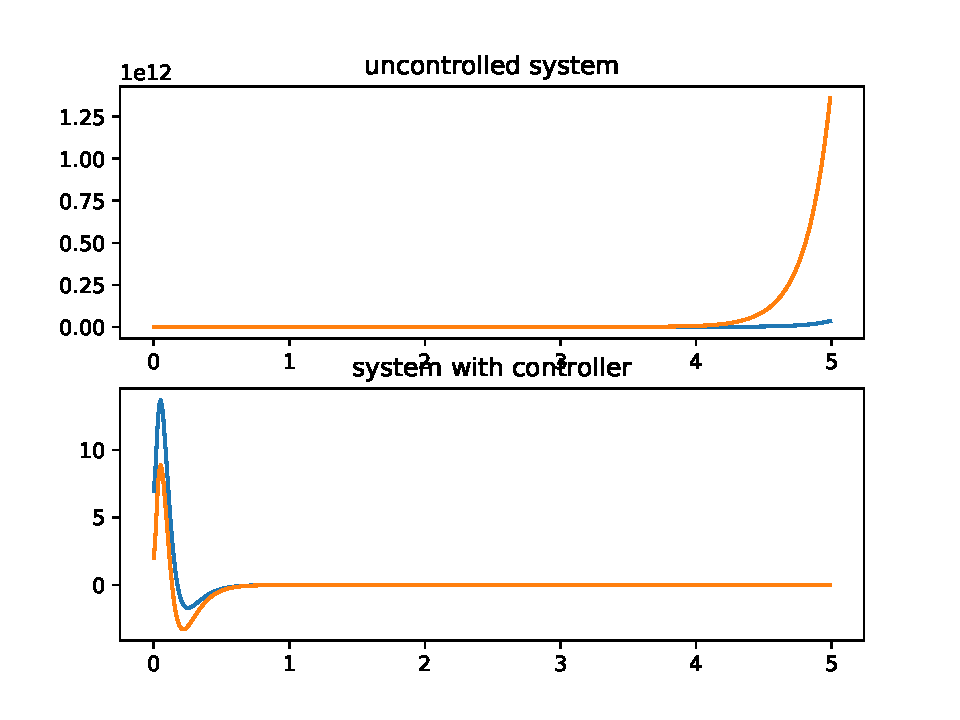
\includegraphics[width=\linewidth]{../Task2/out.pdf}
\end{center}

\section{Used software}
\begin{itemize}
    \item Python 3.8.1
    \item Matlab R2018b 9.5.0
    \item draw.io
\end{itemize}
All software was run under Manjaro Linux with 5.4.18-rt kernel
\section{References}
\begin{itemize}
    \item \href{https://ocw.mit.edu/courses/aeronautics-and-astronautics/16-30-feedback-control-systems-fall-2010/lecture-notes/MIT16_30F10_lec14.pdf}
    {MIT OpenCourseWare}
\end{itemize}
\end{document}